\documentclass[a4paper,12pt]{report}

%\usepackage{extsizes}
\usepackage{cmap}
\usepackage[utf8]{inputenc} %Кодировка файла 
\usepackage[T2A]{fontenc} %корректное отображение русских шрифтов
\usepackage[english, russian]{babel} %переносы слов
\usepackage{fancyvrb}

%for lcov
\usepackage{lscape} %landspace
\usepackage{float}
\usepackage{tabu}
\usepackage{booktabs}
\usepackage{xcolor}
\definecolor{coverage_Hi}{rgb}{0, 1, 0}
\definecolor{coverage_Med}{rgb}{1, 1, 0}
\definecolor{coverage_Lo}{rgb}{1, 0, 0}
\definecolor{cov_cov}{rgb}{0.9,0.9,1}
\definecolor{cov_diff}{rgb}{1,1,0.5}
\definecolor{cov_nocov}{rgb}{1,0.5,0.5}
\definecolor{cov_nop}{rgb}{0.95,0.95,0.95}
\usepackage{listings}
\usepackage{picture}

\usepackage{graphicx}

%\linespread{1.3}
\renewcommand{\rmdefault}{ftm}
%\frenchspacing

%TimeNewRoman
%\usepackage{fontspec}
%\setmainfont[Mapping=tex-text]{Times New Roman}

%Поля
\usepackage{geometry}
\geometry{left=3cm}
\geometry{right=1.5cm}
\geometry{top=2.4cm}
\geometry{bottom=2.4cm}

\usepackage{verbatim}
\usepackage{spverbatim}
\renewenvironment{lstlisting}{\spverbatim}{\endverbatim}

%\renewcommand{\labelenumii}{\arabic{enumi}.\arabic{enumii}.} %стиль нумерованных списокв

\title{SMTP сервер\textnumero 1}
\author{(Агеев~А.~В.)}

\begin{document}
	\maketitle

	\tableofcontents

	\addcontentsline{toc}{chapter}{Введение}
	\chapter*{Введение}
	Для функционирования компьютерных сетей, на оборудовании устанавливается программное обеспечение реализующий различные протоколы взаимодействия. Протоколы различаются по назначению. В данное время для обеспечения сети интернет используется стек протоколов TCP/IP, который состоит из протоколов выполняющий каждый свою задачу:
	\begin{itemize}
		\item Канальный уровень (например Ethernet)~--~беспечивают отправку и прием данных данных через среду передачи.
		\item Сетевой уровень (ip)~--~Канальный уровень работает с множеством устройств, которые объединены в одну группу (сеть). В данной группе устройства <<видят>> друг друга напрямую. Протоколы сетевого уровня предназанчены для обеспечения взаимодействия устройст из разных групп. Две сети объединяются маршрутизатором, а с помощью протокола сетевого уровня выплняется адресация устройст. В этом случае, между устройствами разных групп существует посредник -- маршрутизатор
		\item Транспортный уровень (TCP, UDP) -- на современном оборудовании работает множество программ, для определения того, какой программе адресованы прешедшые данные из сети, используются протоклы транспротного уровня. Их основная цель -- адресация процессов на устройстве.
		\item Прикладной уровень -- данные протоколы реализуются приложениями, которую выполняют некоторую задачу. 
	\end{itemize}

	Целью курсовой работы является реализация протокола прикладоного уровня для получения и доставки электронной почты -- Simple Mail Transfer Protocol (SMTP). А именно, части, которая выполняет прием почты и выполняет ее передачу на следующий этап -- отправку почты.

	\chapter{Аналитический раздел}

	\section{Основные понятия протокола SMTP}

	 SMTP протокол основан на клиент-серверной архитектуре. В данном случае клиентом выступает программа, которая хочет отправить почту, а сервером является программа для приема почты. Протокол поддреживает маршрутизацию почты, то есть серверу может придти письмо, которое адресовано клиенту на другом сервере. В этом случае серверное программное обеспечение принимает роль клиента и отправлет почту другому серверу. 

	 Протокол состоит из текстовых сообщений, которые передают друг другу клиент и сервер при взаимодействии. Каждое сообщение прдеставляет из себя команду с параметрами, которые выполняются сервером. На какждую команду серверв выдает отклик. При организации надежного соединения (например посредством протокола TCP) клиент инициирует почтову транзакцию, которая состоит из последовательности команд, задающих отправителя и получателя сообщения, а так же передается содержательная часть письма. После чего клиент может завершить сеанс или начать новую почтовую транзакцию для передачи очередного письма.

	 \underline{Объекты электронной почты:} (\{Конверт; Содержимое\})
	 \begin{itemize}
	 	\item Конверт
	 	   \begin{itemize}
	 	       \item Адрес отправителя -- определяется командой \textit{MAIL FROM}, которая так же начинает почтовую транзакцию. 
	 	       \item Адрес получателей - с помощью команды \textit{RCPT TO} определяется один получатель и маршрут почты до этого получателя (в RFC2821 указано, что лучше механизм маршрутизации почты игнорировать). Данная команда может быть передана несоклько раз для указания списка получателей одного письма.
	 	       \item Дополнительные заголовки. Протокол SMTP поддреживает расширения - добавление новых заголовков и параметров к стандартным заголовкам.
	 	   \end{itemize}
	 	  \item Содержимое -- передается после отправки команды \textit{DATA}
	 	  \begin{itemize}
	 	      \item Заголовок - список полей вида <ключ>:<значение>, спецификация которых описана в RFC5322
	 	      \item Тело сообщения - это непосредственное содержимое письма, которая представляет из себя текстовый набор данных соответсвущий спецификации форматов разны типов объектов MIME (Multipurpose Internet Mail Extensions)
	 	  \end{itemize}
	 \end{itemize}
	 Все элементы описваются с исопльзованием 7-битной кодировки US-ASCII, но это ограничение может быть снято с использованием расширения протокола \textit{8BITMIE}
	
	 \underline{Получатель и отправитель:}
	 
	 Протокол SMTP работает в 2 стороны. Получателем и отправителем может выступать как почтовая служба на сервере так и клиентское программное обеспечение. В протоколе выделяются следующие понятия:
	 \begin{itemize}
	     \item Клиент -- Отправлющая сторона в текущей почтовой транзакции.
	     \item Сервер -- Принимающая сторона в текущей почтовой транзации.
	     \item Агент доставки почты (Mail Transfer Agent, MTA)~-- Клиент и сервер SMTP обеспечивающее почтовый трансопртный сервис.
	     \item Пользовательский почтовый агент (Mail User Agent, MUA)~-- Программное обеспечение выступающее в качетсве исходных отправителей и конечных получателей почтовых сообщений
	 \end{itemize}
	 $$MUA\rightarrow MTA \rightarrow MTA \rightarrow MUA$$
	 
	 \underline{Типы агентов SMTP:}
	 
	 \begin{itemize}
	     \item Система отрпавки (originator) -- Вносит сообщение в среду передачи данных, в котором находится транспортный сервис.
	     \item Система доставки (delivery) -- Принимает почту от транспортного серивса и передает ее пользовательскому агенту или размещает ее в хранилище.
	     \item Транслятор (relay) -- Получает почту от клиента и передает ее другому серверу.
	     \item Шлюз (gateway) -- Система получающие письма от одной транспортной среды и передающие письма сереверу находящейся в другой транспортной среде.
	 \end{itemize}
	 
	 
	 \section{SMTP сеанс}
	 
	 При подключении клиента к серверу начинается SMTP сеанс, в течении которого выполняется взаимодействие клиента и сервера по доставки писем.
	 \begin{enumerate}
	     \item Инициирование соединения 
	     
	     Клиент: создает соединение с сервером
	     
	     Сервер: Отправляет отклик
	     \begin{itemize}
	         \item 220 в случае готовности
	         \item 554 в случае отказа в SMTP сервисе
	     \end{itemize}
	     \item Инициирование клиента (сеанса)
	     
	     Клиент: передает команду \textit{HELO/EHLO}. \textit{HELO} - содание SMTP сеанса. \textit{EHLO} - создание SMTP сеанса с поддержкой расширений протокола (Extend Hello).
	     
	     Сревер: Отрпавляет отклик 250. Если бла отправлена команда \textit{EHLO}, то сервер так же возращает список расширений, который он поддерживает (расширения далее не рассматриваются)
	     
	     \item Почтовая транзакция (Транзакцию нельзя сделать вложеной в другую транзакцию)
	     \begin{enumerate}
	         \item \label{item:mail_transaction} Начало транзакции
	         
	         Клиент: Отправлет команду \textit{MAIL FROM}. Команда говорит о запуске новой почтовой транзакции и передает адрес отправителя. Если в процессе передачи возникнет ошибка, на этот адрес будет отправлено уведомление.
	         
	         Сервер: Отклик 250
	         
	         \item Определение спика получателей
	         
	         Для определение списка получателей клиент отправлет несколько команд \textit{RCPT TO}, на каждую из которых сервер отправляет отклик 250.
	         
	         Если команда \textit{RCPT TO} отправлена до начала почтовой транзакции, то сервер отправлет отклик 503
	         
	         \item Передача тела письма 
	         
	         Клиент: Отправлет команду \textit{DATA} 
	         
	         Сервер: отправлет отклик 354, что свидетельствует о том, что сервер готов принимать содержимое письма
	         
	         Клиент: Отрпавлет все почтовые данные. После завершения отправки тела письма, клиент должен отправить точку на отдельной строке (<CRLF>.<CRLF>~--~послеовательность кончания данных письма)
	         
	         Сервер: Должен воспринимать все присилаемые данные, как тело письма. Как только он получает последовательность конца данных (<CRLF>.<CRLF>) сервер должен инициировать процесс доставки письма. А клиенту отправить отклик 250
	     \end{enumerate}
	     
	     \item Завершение сеанса или новая транзакция
	     \begin{itemize}
	         \item Если клиент желает завершить работу с сервером, то он должен послеть команду \textit{QUIT}, на которую сервер должен ответить откликом 221 и закрыть соединение.
	         \item Если клиент желает продолжить работу с сервером, то он должен создать новую почтовую транзакцию. Для этого необходимо перейти на шаг \ref{item:mail_transaction}
	     \end{itemize}
	 \end{enumerate}
	 
	 \underline{Дополнительные команды:}
	 \begin{enumerate}
	     \item \textit{VRFY}
	     \item \textit{EXPN}
	     \item \textit{RSET} -- прерывание текущей почтовой транзакции. Отклик сервера: 250
	     \item \textit{HELP}
	     \item \textit{NOOP}
	 \end{enumerate}
	 
	 \section{Синтаксис команд}
	 \begin{verbatim}
ehlo = "EHLO" SP Domain CRLF
helo = "HELO" SP Domain CRLF
ehlo-ok-rsp  = ("250" domain [SP ehlo-greet] CRLF)
              | ("250-" domain [SP ehlo-greet] CRLF
              | *("250-" ehlo-line CRLF)
              | ("250" SP ehlo-line CRLF)

ehlo-greet = 1*(%d0-9 / %d11-12 / %d14-127)
ehlo-line = ehlo-keyword *( SP ehlo-param )
ehlo-keyword = (ALPHA / DIGIT) *(ALPHA / DIGIT / "-")
ehlo-param   = 1*(%d33-127)
"MAIL FROM:" ("<>" / Reverse-Path) [SP Mail-parameters] CRLF
"RCPT TO:" ("<Postmaster@" domain ">" /
           "<Postmaster>" / Forward-Path) 
           [SP Rcpt-parameters] CRLF
"DATA" CRLF
"RSET" CRLF
"VRFY" SP String CRLF
"EXPN" SP String CRLF
"HELP" [ SP String ] CRLF
"NOOP" [ SP String ] CRLF
"QUIT" CRLF
Reverse-path = Path
Forward-path = Path
Path = "<" [ A-d-l ":" ] Mailbox ">"
A-d-l = At-domain *( "," A-d-l )
At-domain = "@" domain
Mail-parameters = esmtp-param *(SP esmtp-param)
Rcpt-parameters = esmtp-param *(SP esmtp-param)
esmtp-param     = esmtp-keyword ["=" esmtp-value]
esmtp-keyword   = (ALPHA / DIGIT) *(ALPHA / DIGIT / "-")
esmtp-value     = 1*(%d33-60 / %d62-127)
Keyword  = Ldh-str
Argument = Atom
Domain = (sub-domain 1*("." sub-domain)) / address-literal
sub-domain = Let-dig [Ldh-str]
address-literal = "[" IPv4-address-literal / 
                      IPv6-address-literal /
                      General-address-literal "]"
Mailbox         = Local-part "@" Domain
Local-part      = Dot-string / Quoted-string
Dot-string      = Atom *("." Atom)
Atom            = 1*atext
Quoted-string   = DQUOTE *qcontent DQUOTE
String          = Atom / Quoted-string
IPv4-address-literal    = Snum 3("." Snum)
IPv6-address-literal    = "IPv6:" IPv6-addr
General-address-literal = Standardized-tag ":" 1*dcontent
Standardized-tag        = Ldh-str
Snum                    = 1*3DIGIT
Let-dig                 = ALPHA / DIGIT
Ldh-str                 = *( ALPHA / DIGIT / "-" ) Let-dig
IPv6-addr               = IPv6-full / IPv6-comp / IPv6v4-full / IPv6v4-comp
IPv6-hex  = 1*4HEXDIG
IPv6-full = IPv6-hex 7(":" IPv6-hex)
IPv6-comp = [IPv6-hex *5(":" IPv6-hex)] "::" [IPv6-hex *5(":"IPv6-hex)]
IPv6v4-full = IPv6-hex 5(":" IPv6-hex) ":" IPv4-address-literal
IPv6v4-comp = [IPv6-hex *3(":" IPv6-hex)] "::"
              [IPv6-hex *3(":" IPv6-hex) ":"] IPv4-address-literal

	 \end{verbatim}
	\section{Тестирование}
		Для тестирования функциональности сервера, было написаны unit-тесты
		с использованием библиотеки cunit. Резултат работы тестиованяи представлен
		в листинге 
		\VerbatimInput{./include/unit_test_out.tex}
		\VerbatimInput{./include/valgrind_out.tex}
		
		Так же было выполнено системное тестирование
		отчет по покрытию тестами представлен в следующей таблице
		%\begin{landscape}
		%	\input{./include/lcov/index}
		%\end{landscape}
		Отчет по покрытию тестами не строится в  gitlab!

	\begin{figure}
	\centering
	\includegraphics[width=\textwidth]{./include/smtp_fsm.pdf}
	\caption{Конечный автомат протокола SMTP}
	\label{fig:smtp_fsm}
	\end{figure}

	\begin{figure}
	\centering
	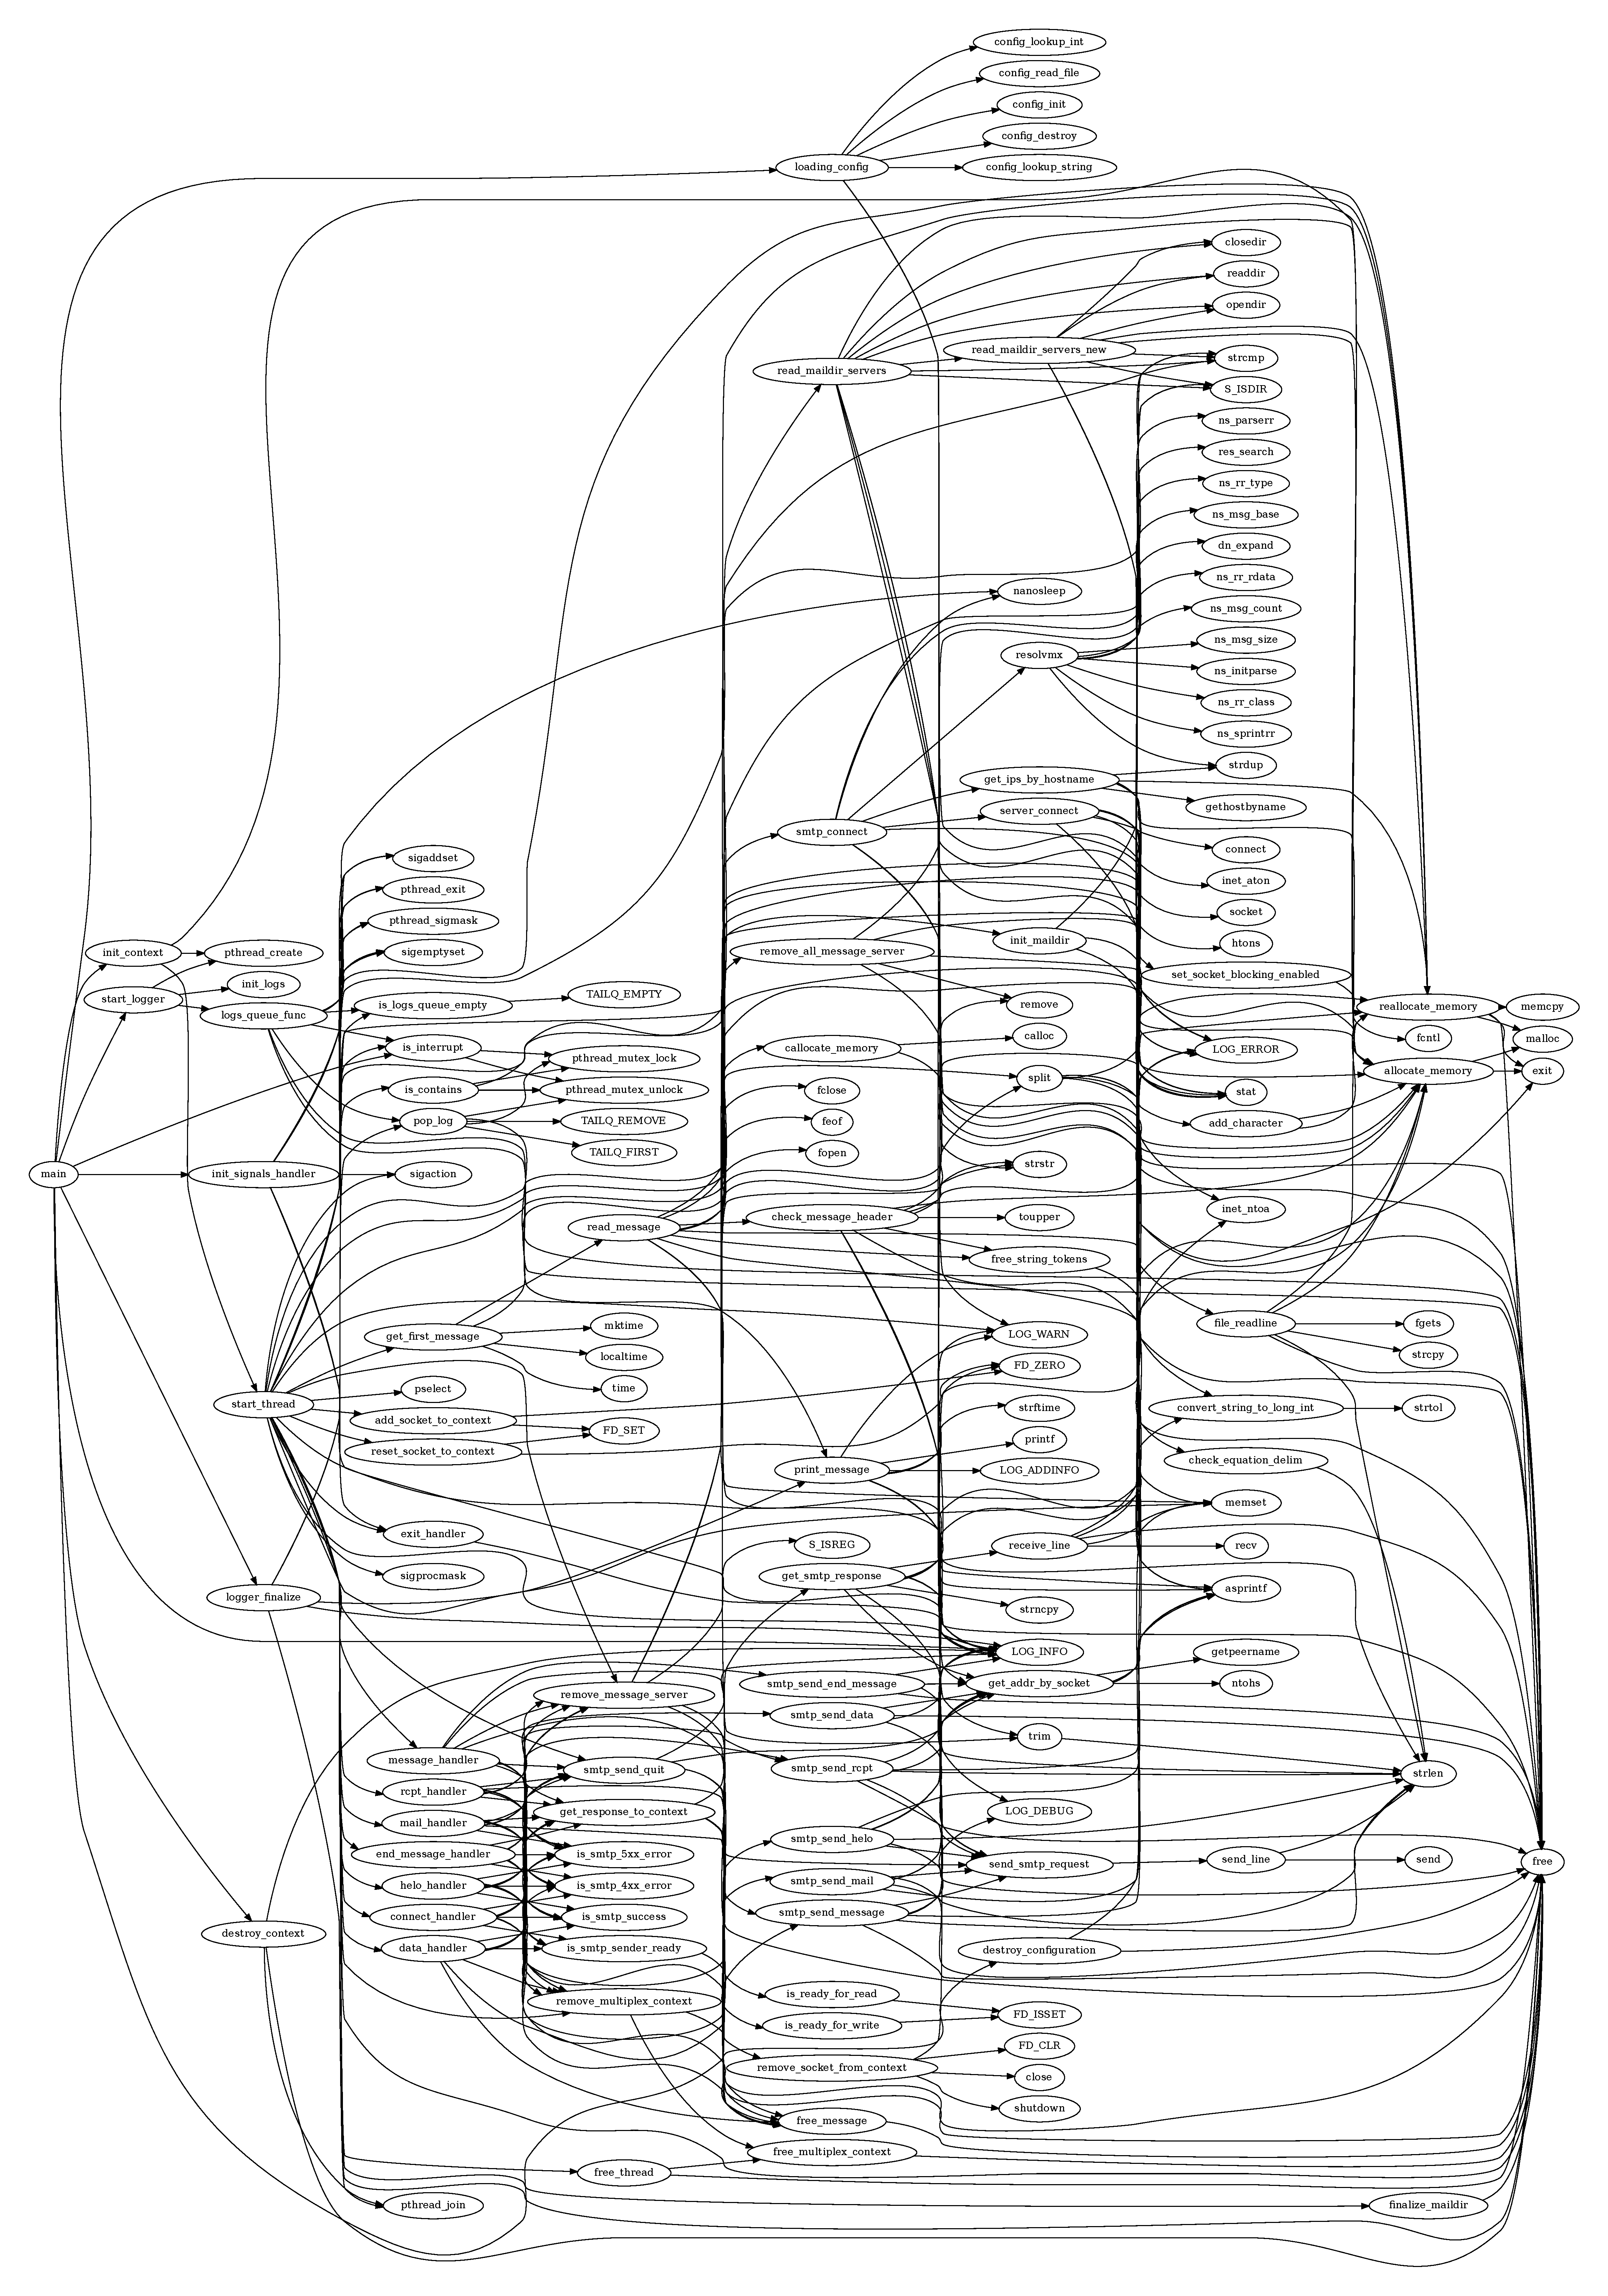
\includegraphics[width=\textwidth]{./include/cflow.pdf}
	\caption{Граф вызовов в модуле EventLoop}
	\label{fig:event}
	\end{figure}

	\begin{figure}
	\centering
	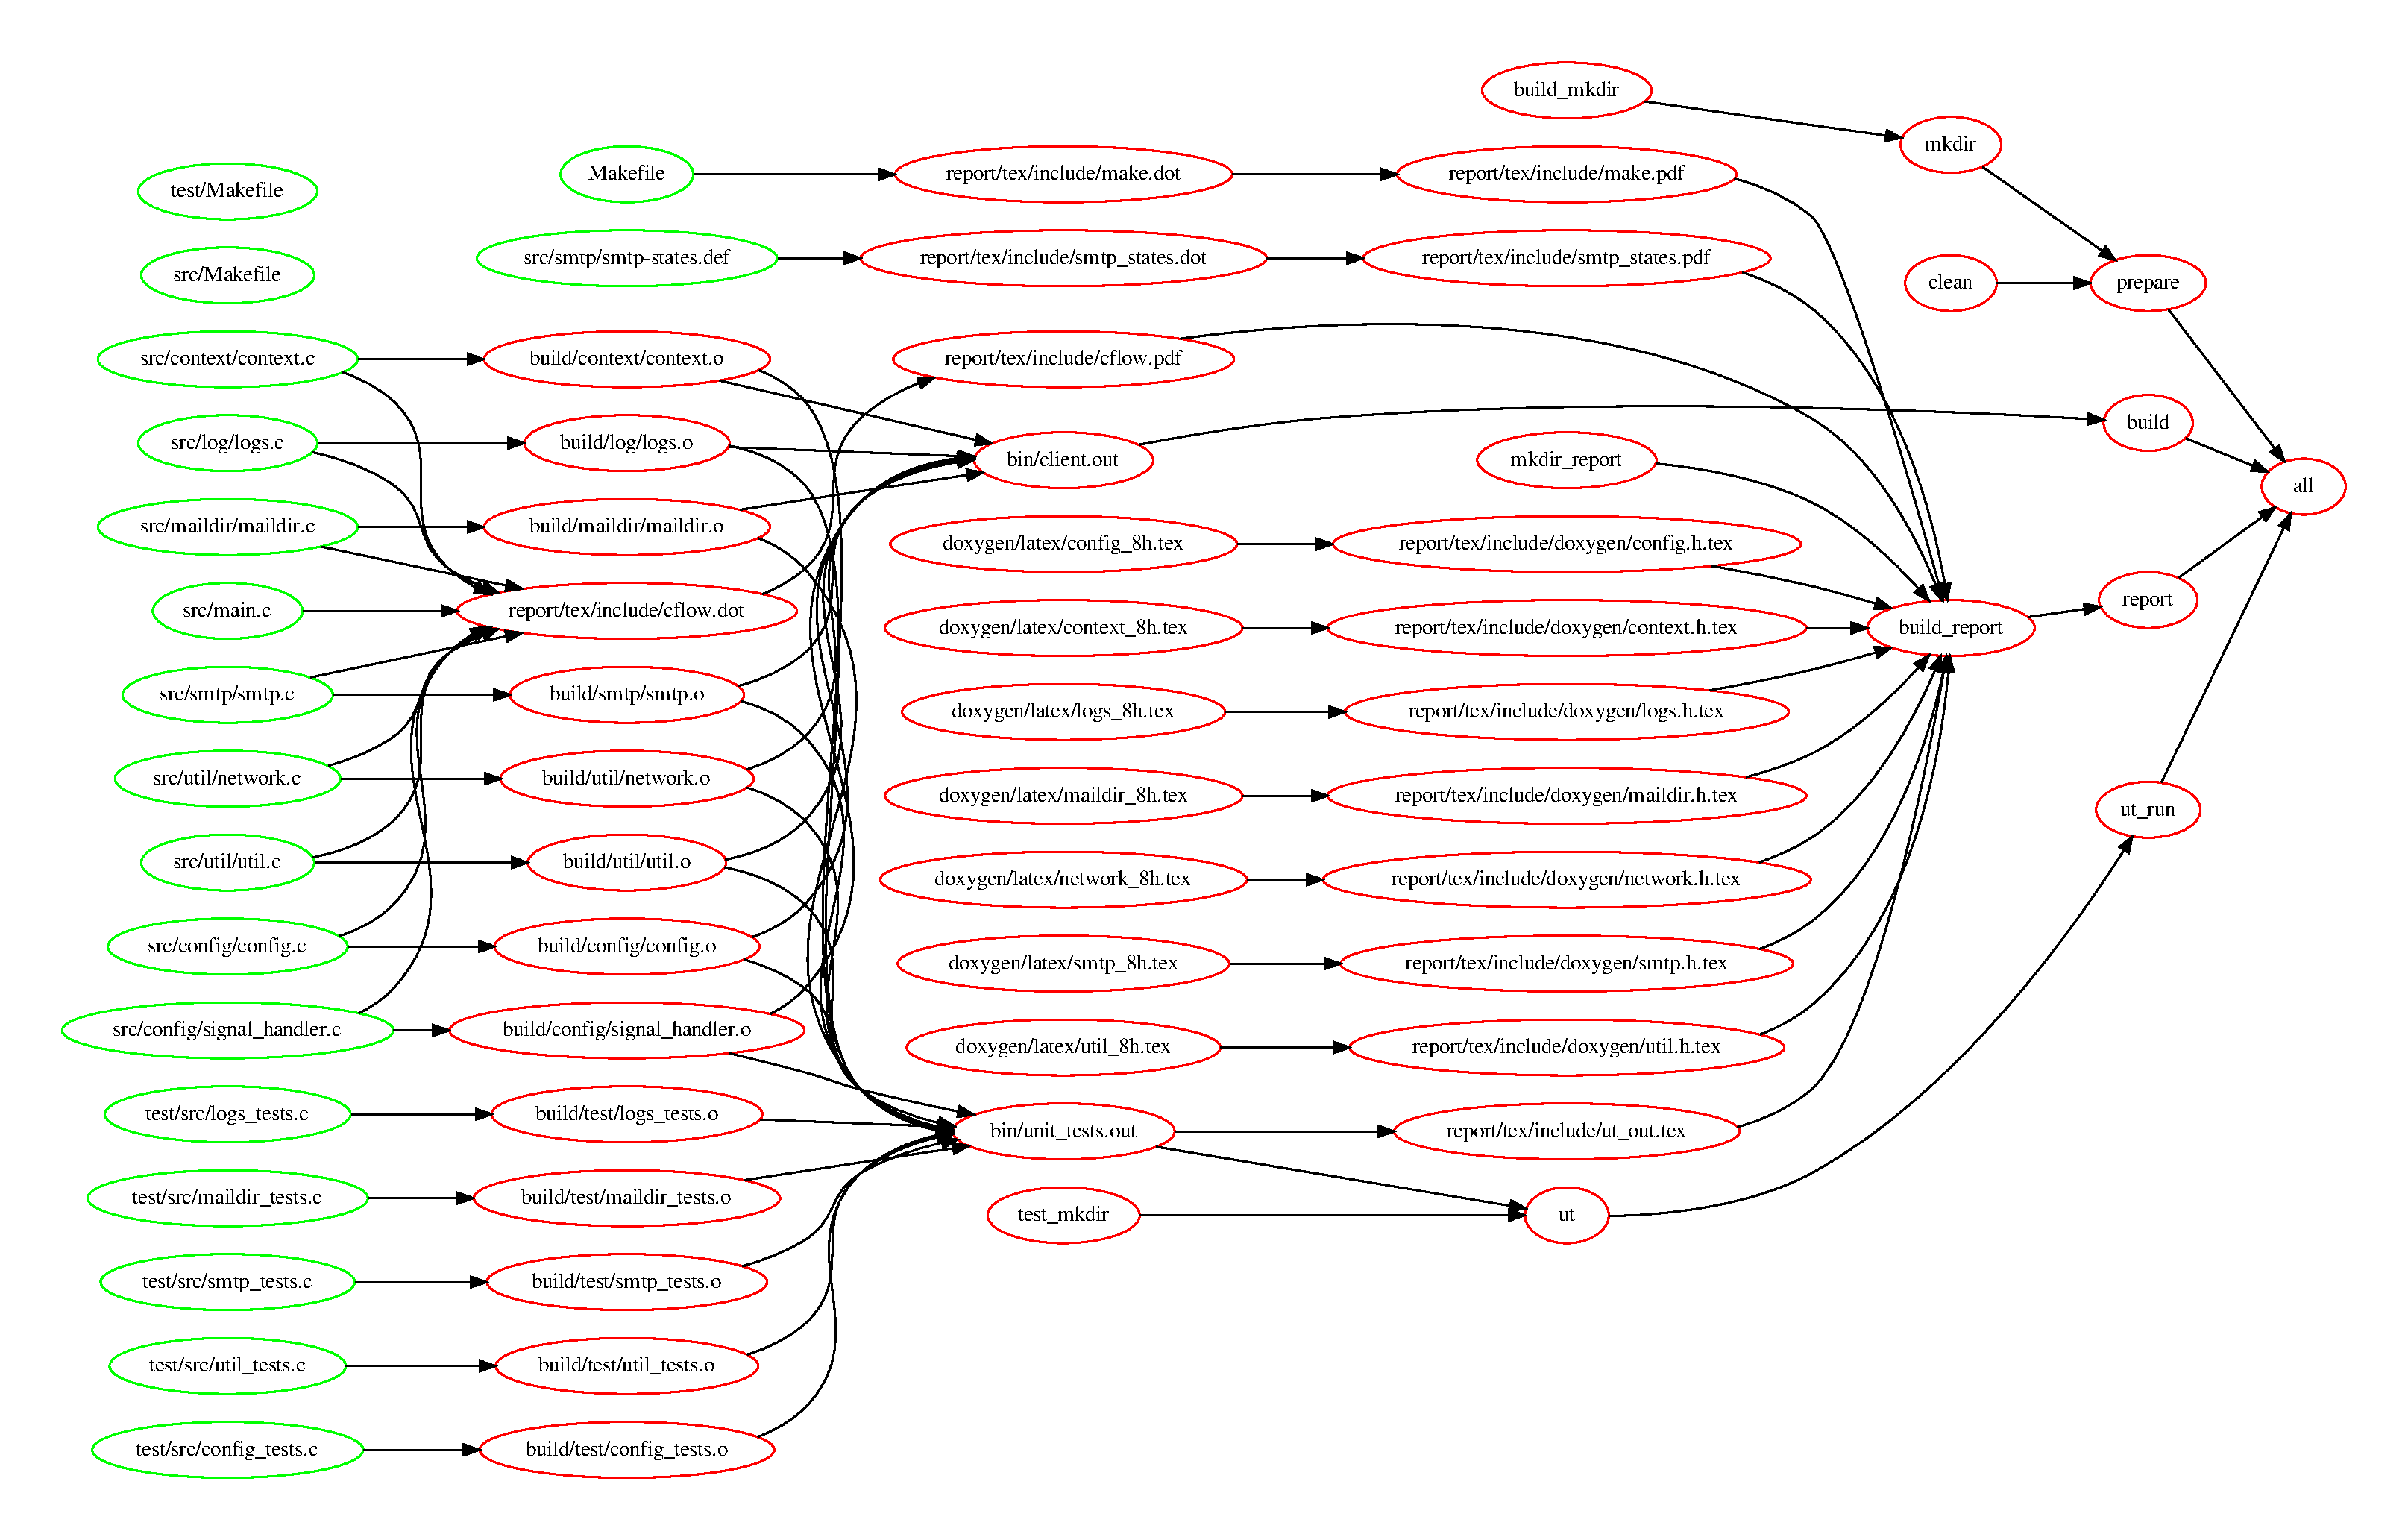
\includegraphics[width=\textwidth]{./include/make.pdf}
	\caption{Структура проекта}
	\label{fig:make_server}
	\end{figure}

	Для реализации smtp протокола использовались регулярные выражения. Которые представленны в следующем листинге
	\include{./include/regex}

	\section{Список источников и литературы}
	\begin{enumerate}
		\item http://rfc.com.ru/rfc2821.htm
		\item http://rfc.com.ru/rfc1123
		\item https://www.protocols.ru/WP/rfc5322/
		\item RFC 1035 DOMAIN NAMES — IMPLEMENTATION AND SPECIFICATION  https://www.protocols.ru/WP/rfc1035/
	\end{enumerate}
\end{document}